\section{Aufbau}
\label{sec:Aufbau}

\begin{figure}
 \centering
 \caption{Eine schematische Darstellung des Messaufbaus}
 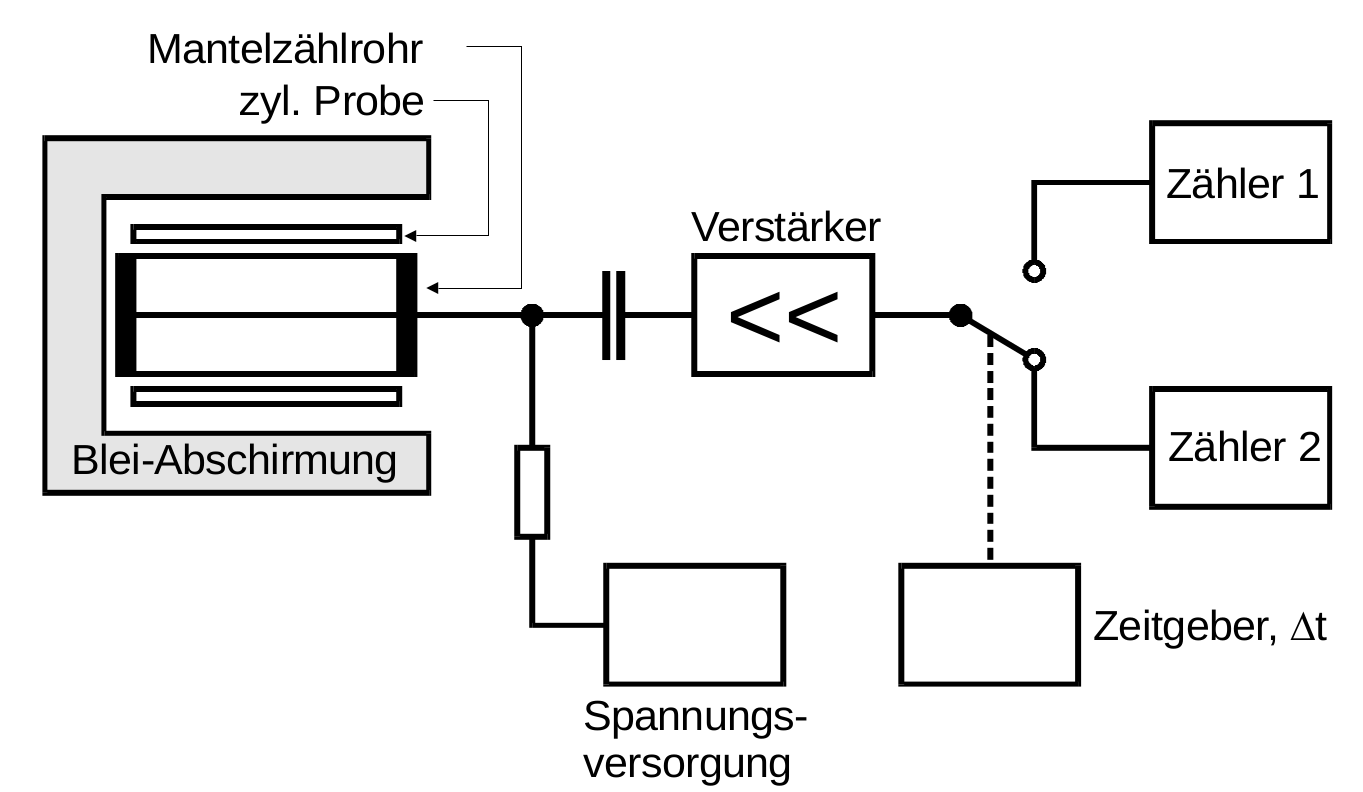
\includegraphics[width=\linewidth-70pt,height=\textheight-70pt,keepaspectratio]{content/aufbau.png}
 \label{fig:aufbau}
\end{figure}

Der Messaufbau besteht im Kern aus einem radioaktiven Isotop und einem Geiger-Müller-Zählrohr, welches entweder auftretende Betateilchen oder Gammaquanten registriert. Zwischen dem Gerät können Metallplatten verschiedener Dicke positioniert werden, welche die Strahlungintensität abschwächen. Die Messzeit kann am Auslesegerät der Trefferzahl eingestellt werden. Zum Schutz vor radioaktiver Strahlung ist der Messaufbau zudem mit einer Bleiverkleidung versehen. 
